\documentclass[conference]{IEEEtran}
\makeatletter
\def\ps@headings{%
\def\@oddhead{\mbox{}\scriptsize\rightmark \hfil \thepage}%
\def\@evenhead{\scriptsize\thepage \hfil \leftmark\mbox{}}%
\def\@oddfoot{}%
\def\@evenfoot{}}
\makeatother
\pagestyle{headings}

\hyphenation{op-tical net-works semi-conduc-tor}


\usepackage{subfigure}
\usepackage{soul}

\usepackage{algorithmic}
\usepackage[ruled,vlined]{algorithm2e}
\usepackage{listings}
\usepackage{color}

\definecolor{dkgreen}{rgb}{0,0.6,0}
\definecolor{gray}{rgb}{0.5,0.5,0.5}
\definecolor{mauve}{rgb}{0.58,0,0.82}

\lstset{frame=tb,
  language=Java,
  aboveskip=3mm,
  belowskip=3mm,
  showstringspaces=false,
  columns=flexible,
  basicstyle={\small\ttfamily},
  numbers=none,
  numberstyle=\tiny\color{gray},
  keywordstyle=\color{blue},
  commentstyle=\color{dkgreen},
  stringstyle=\color{mauve},
  breaklines=true,
  breakatwhitespace=true,
  tabsize=3
}


\usepackage{algorithmic}
\usepackage[ruled,vlined]{algorithm2e}
\usepackage{graphicx}

\if CLASSINFOpdf
  \usepackage[pdftex]{graphicx}
  % declare the path(s) where your graphic files are
  % \graphicspath{{../pdf/}{../jpeg/}}
  % and their extensions so you won't have to specify these with
  % every instance of \includegraphics
  % \DeclareGraphicsExtensions{.pdf,.jpeg,.png}
\else
  % or other class option (dvipsone, dvipdf, if not using dvips). graphicx
  % will default to the driver specified in the system graphics.cfg if no
  % driver is specified.
  % \usepackage[dvips]{graphicx}
  % declare the path(s) where your graphic files are
  % \graphicspath{{../eps/}}
  % and their extensions so you won't have to specify these with
  % every instance of \includegraphics
  % \DeclareGraphicsExtensions{.eps}
\fi
% graphicx was written by David Carlisle and Sebastian Rahtz. It is
% required if you want graphics, photos, etc. graphicx.sty is already
% installed on most LaTeX systems. The latest version and documentation can
% be obtained at:
% http://www.ctan.org/tex-archive/macros/latex/required/graphics/
% Another good source of documentation is "Using Imported Graphics in
% LaTeX2e" by Keith Reckdahl which can be found as epslatex.ps or
% epslatex.pdf at: http://www.ctan.org/tex-archive/info/
%
% latex, and pdflatex in dvi mode, support graphics in encapsulated
% postscript (.eps) format. pdflatex in pdf mode supports graphics
% in .pdf, .jpeg, .png and .mps (metapost) formats. Users should ensure
% that all non-photo figures use a vector format (.eps, .pdf, .mps) and
% not a bitmapped formats (.jpeg, .png). IEEE frowns on bitmapped formats
% which can result in "jaggedy"/blurry rendering of lines and letters as
% well as large increases in file sizes.
%
% You can find documentation about the pdfTeX application at:
% http://www.tug.org/applications/pdftex

\begin{document}
\title{Sistema di rilevamento della presenza di pedoni sulla carreggiata}

% Author names 
% note positions of commas and nonbreaking spaces ( ~ ) LaTeX will not break
% a structure at a ~ so this keeps an author's name from being broken across
% two lines.
% use \thanks{} to gain access to the first footnote area
% a separate \thanks must be used for each paragraph as LaTeX2e's \thanks
% was not built to handle multiple paragraphs
\author{
Simone Bertolini,
Gianmarco Santini,
\\
\IEEEauthorblockA{University of Bologna, Italy \\
 \\
Emails: simone.bertolini@studio.unibo.it, gianmarco.santini@studio.unibo.it}}




% make the title area
\maketitle

% The Abstract
\begin{abstract}
La mortalit\'a stradale \'e un problema molto importante nella nostra comunit\'a, ogni anno per le strade ci sono circa 3.283 vittime (morti entro il 30° giorno) e 249.175 feriti. Una delle cause principali \'e sicuramente la distrazione da parte di chi guida. Noi proponiamo un sistema di rilevamento di collisione in grado di avvisare il conducente della presenza di un pedone che gli attraverser\'a la strada. Tale sistema \'e soggetto a vincoli importanti in quanto la localizzazione di una persona pu\'o richiedere un consumo di energia proibitivo da parte dello smartphone e il raggio di rilevamento dei dispositivi \'e limitata. Il nostro sistema \'e pensato come un'estensione per un sistema di navigazione come google maps in modo da poter avvisare il conducente direttamente sulla mappa dove si trover\'a il pedone. Come verr\'a descritto in seguito tale sistema comprende due modalit\'a di funzionamento la prima dedicata al pedone e la seconda dedicata al conducente di un veicolo. La comunicazione tra i vari dispositivi avviene tramite Wi-Fi Direct e la localizzazione del pedone avviene tramite l'uso congiunto di GPS e i sensori dello smartphone.

\end{abstract}



\section{Introduzione}
Una delle cause principali di mortalit\'a in italia sono sicuramente gli incidenti stradali, questi ogni anno mietono migliaia di persone e costituiscono sicuramente un problema importante. Nel 2017 sono stati 174.933 gli incidenti stradali con lesioni a persone, con 3.378 vittime (morti entro 30 giorni dall'evento) e 246.750 feriti. Tra questi sono presenti i pedoni investiti da automibilisti distratti alla guida che non si accorgono della loro presenza finch\'e non \'e troppo tardi. Questo \'e il problema che il nostro sistema cerca di risolvere, di seguito nel capitolo II vengono descritte tecnologie e metodi che hanno contribuito alla pianificazione e sviluppo del sistema, nel capitolo III viene descritta l'architettura dell'applicazione e il funzionamento, nel capitolo IV viene descritta l'implementazione, nel capitolo V vengono analizzate le performance e infine nel capitolo VI vengono tratte le nostre conclusioni.  
(da togliere poi)Descrivi qui il contesto generale, i contributi del progetto, e la struttura del documento.
 

\section{Related works}
In questa sezione vengono descritti metodologie e strutture che hanno aiutato allo sviluppo del sistema. \cite{ref1}  Descrive un sistema a basso costo e consumo per la localizzazione continua di un dispositivo con buona accuratezza, questo sistema fa uso di GPS in concomitanza con accelerometro, giroscopio e magnetometro in modo da ridurre i consumi sui dispositivi interessati. Tale sistema per\'o \'e dedicato a una localizzazione della persona non solo all'esterno ma anche all'interno di edifici, mentre il nostro si occupa solo della localizzazione all'esterno. \cite{ref2} Descrive un'algoritmo per tracciare e localizzare un veicolo in tempo reale utilizzando GPS, accelerometro e giroscopio su uno smartphone con sistema android. Tale algoritmo è in grado rispondere ai cambi di velocit\'a e di direzione in tempo reale senza avere informazione dal GPS. \cite{ref3} Illustra un sistema per il tracciamento di percorsi di guida ibrido che utilizza barometro, GPS, accelerometro e giroscopio cercando di ridurre i consumi energetici dello smartphone. Tale sistema \'e pensato per misurare gli spostamenti dello smartphone in modo continuo e per identificare certi spostamenti conosciuti che le persone ripetono più spesso. Infine \cite{ref4} descrive in modo completo il funzionamento e l'implementazione dell'architettura Wi-Fi direct che come verr\'a descritto successivamente \'e quella che \'e stata utilizzata per lo sviluppo del nostro sistema. 
Fornisci una breve rassegna di articoli di ricerca, software, prototipi o tecnologie che sono collegate in qualche modo al problema affrontato nel progetto. Tutti i lavori devono essere referenziati ed inseriti nella Bibliografia.

\section{Architettura}
Il sistema \'e stato progettato per funzionare su ambiente Android, permetttendo in questo modo di essere utilizzato in larga scala e senza costi aggiuntivi al prezzo del dispositivo stesso. Tale sistema \'e costituito da due tipologie di layer applicativi che potremmo denominare come Publisher e Observer, cos\'i da poter rendere il pi\'u intuitivo possibile il ruolo da loro ricoperto.
\begin{figure}[ht!]
	\centering
	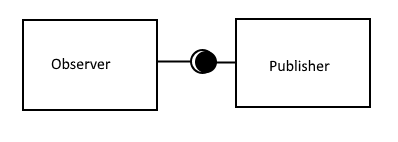
\includegraphics[width=0.7\linewidth]{ps}
	\caption{Concetti base}
	\label{fig:ps}
\end{figure}
\\
Il ruolo del Publisher viene assunto da tutti i dispositivi in possesso ai pedoni, il loro compito principale \'e quello di avvisare i veicoli circostanti riguardo la propria posizione corrente e la direzione in cui si stanno muovendo. Tutti i veicoli presenti sulla strada, invece, assumono il ruolo di Observer ed hanno il compito di ascoltare in ogni istante i Publisher, elaborare i loro dati e avvertire i conducenti in caso di pericolo. La struttura della rete risulta dunque essere un insieme approsimatamente omogeneo di Publisher ed Observer. La forza di questo sistema è il fatto che la rete non preveda una vera e propria sturuttra, ma che si adatti a quelle che sono le limitazioni dell'ambiente circostante. Questa qualità del sistema lo rende flessibile e particolarmente scalabile.

\section{Implementazione}
L'applicazione \'e divisa in due modalit\'a, Publisher e quella Observer. La prima \'e quella relativa al pedone che si occupa di tracciare i suoi movimenti, la sua velocit\'a e la sua direzione di movimento. La seconda quella del veicolo che si occupa di elaborare le informazione fornite dai pedoni e stimare in base ad esse se sar\'a presente una collisione. Di seguito verranno descritte le informazioni e i vari passaggi che hanno portato allo sviluppo dell'applicazione.

\subsection{Ambiente di Sviluppo}
Come gi\'a descritto in precedenza, il sistema \'e stato completamente sviluppato per sistema operativo Android in modo da consentire la maggior portabilit\'a del software. Infatti il nostro obiettivo non era solo la verifica verticale delle funzionalit\'a del software, ma anche il confronto orizzontale tra dispositivi che utilizzano hardware differenti. Questo ha consentito di trovare i punti in comune ma anche le discrepanze tra i diversi dispositivi hardware e di generare un software flessibile in grado di adattarsi al dispositivo host. Per lo sviluppo  \'e stato utilizzato l'IDE di default di Android ovvero Android Studio con linguaggio di programmazione Java.

\subsection{Obiettivi}
L'idea iniziale era quella di riuscire ad inidividuare un pedone con il maggior preavviso possibile, ma limitando il consumo energetico del dispositivo ad egli in possesso. Per fare ci\'o abbiamo effettuato alcuni test utilizzando il Bluetooth, la tecnologia a radio frequenza con il miglior risparmio energetico. In particolare ci siamo concentrati sull'utilizzo dei Beacon Bluetooth inviati dal dispositivo pedone ed elaborati dal veicolo. Al loro interno sono stati inseriti dati fittizi che simulassero un payload di dimensioni verosimili. Le prove effettuate includevano l'invio dei beacon sia dal veicolo in movimento che dal pedone a velocit\'a ridotta. Purtroppo in entrambi casi i risulati ottenuti sono notevolmente scadenti. Infatti i dispositivi riuscivano a trovarsi solo a distanze quasi nulle (non pi\'u di una decina di metri). La nostra seconda scelta \'a dunque ricaduta sull'utilizzo del WiFi Direct(P2P). Nel paragrafo seguente vedremo in breve come funziona questo standard.

\subsection{WiFi Direct e Problemi riscontrati}
Wi-Fi Direct (nato con il nome Wi-Fi P2P - Wi-Fi Peer-to-Peer) \'e uno standard della Wi-Fi Alliance, ormai comune in molti prodotti come smartphone, tablet, stampanti, videocamere digitali, console di gioco e scanner, che consente a due o più dispositivi certificati di connettersi tra loro con un collegamento Wi-Fi diretto senza aver bisogno di un router wireless o di un hotspot. In particolare questa tecnologia prevede 3 fasi prima dio poter scambiare dati:
\\
1) Effettuare il discovery dei dispositivi circastanti
\\
2) Creazione di un gruppo (se questo non esiste gi\'a) al fine di poter poi accettare la connesione
\\
3) Effettuare handshake di connessione

Come racconta lo standar IEEE, il WiFi P2P garantisce una riuscita della connessione all'interno del range dei 13 secondi. Purtroppo, per il nostro applicativo queste latenze sarebbero state enormi ed avrebbero reso il sistema inutilizzabile.
Abbiamo dunque deciso di sviluppare un applicazione di chat base, che ci aiutasse a stimare il reale tempo di riuscita della connessione tra due dispositivi.
I test ci hanno riportato quanto segue:
\\
- Tempo di connessione ~3/4,\\
- Una volta stabilita la connessione il tempo di risposta ad un messaggio era pressoch\'e nullo.
I 3-4 di connessione non rispecchiavano in tutto per tutto le nostre esigenze in quanto, non certi del range del segnale WiFi, 3s * (50km/h / 3.6) =~40m di range sarebbero stati persi in partenza.

Non potendo consentire la connessione tra i dispositivi, ci rimaneva unicamente la fase di Discovery da sfruttare.
All'interno del record di Discovery, infatti, vi si pu\'o inserire qualunque dato sottoforma di tabella hash ed il processo di segnalazione e di ricezione del segnale \'e pressoch\'e immediato.
Fatte queste considerazioni, abbiamo deciso di demolire l'applicazione di chat lasciando unicamente la parte di discovery ed effettuare svariati test in cui misuravamano la distanza minima in cui i due dispositivi riuscivano a vedersi per la prima volta.
I riusultati sono stati eccezionali. Infatti i valori in metri ottenuti sono stati da un centinaio di metri in campo aperto a 45-50 metri in curva con traiettoria in linea d'aria offuscata da ostacoli.
Questo principio \'e risultato per noi essere le fondamenta vere e proprie del sistema stesso.
Sfortunatamente le librerie di android non funzionano molto bene per quanto riguarda il publishing ed il discovery nel WiFi Direct. Infatti se si vuol pubblicare i propri dati sulla rete bisogna anche effettuare un'operazione continua di Discovery, altrimenti nessuno dato viene spedito. Inoltre (considerando che il Discovery chiama una callback ogni volta che trova un dispoositivo) la callback del Discovery non segnala lo stesso dispositivo pi\'u di una volta se esso \'e gi\'a stato trovato anche se possiede un record differente.
Questo ci ha costretti a resettare la procedura del discovery ogni T secondi in modo da poter mettere il dispositivo Observer nuovamente in ascolto anche di Pubblisher gi\'a trovati.
Per valori di T inferiori ai 7-8 secondi si rischia di mandare in crash il driver del modulo WiFi che, non so se per problemi interni o per verifiche di funzionamento del sistema operativo, viene disattivato bloccando qualsiasi forma di ricezione e/o trasmissione.
L'applicativo lato publisher fornisce all'interno del proprio record di service discovery i seguenti dati che varrannoo poi discussi nei paragrafici successivi nei relativi modelli.\\
- Longitudine\\
- Latitudine\\
- Velocita\\
- Timestamp\\
- Timestamp della Posizione\\
- Accuratezza\\
- Bearing\\
Lato Observer invece, i dati di tutti i pedoni trovati tramite il discovery vengono salvati (eventualmente aggiornati se gia trovati in precedenza), processati ed alla fine del loro ciclo vita eliminati.


\subsection{Test Effettuati}
Per quanto riguarda la localizzazione del pedone l'idea \'e stata quella di usare il GPS unito ai sensori dello smartphone in modo da ottentere una localizzazione abbastanza precisa con un consumo energetico contenuto. A questo proposito \'e stato necessario eseguire qualche test per controllare quali output i vari sensori fornissero e come utilizzare quest'ultimi. In particolare \'e stato necessario suffermarsi sul rotation vector, in quanto ci serviva la direzione in cui il pedone sta camminando, per controllare quanto preciso era il calcolo dell'azimuth, l'angolo relativo al nord magnetico. Quest'angolo \'e risultato essere molto sensibile cio\'e, il valore non rimaneva fisso ma tendeva a cambiare al minimo movimento dello smartphone. Altri test sono stati eseguiti con lo step counter, il sensore che dovrebbe segnalare ogni volta che viene effettuato un passo, esso \'e risultato essere un p\'o inpreciso nei passi corti e nei cambi di direzione dove a volte segnava dei passi non effettuati. Inoltre le segnalazione della presenza di un passo non era immediata ma poteva accadere che venisse segnalata dopo aver effettuato un nuovo passo indicando la presenza di entrambi. 

\subsection{Modello di Localizzazione}
Di seguito viene descritto come avviene la localizzazione del pedone e come vengono calcolati i vari dati da inviare tramite Wi-Fi direct ai vari veicoli presenti nel range di trasmissione. La classe che si occupa di fare ci\'o \'e la classe HumanLocalService, tale classe sfrutta i valori dei sensori rotation vector e step detector per stimare la posizione del pedone. Al''interno del costruttore infatti vengono implementati i vari listener che si occupano di eseguire delle operazione nel momento in cui avviene un aggiornamento nei dati rilevati dai sensori. 
Qui sotto \'e possibile osservare il codice relativo al listener del sensore rotaion vector, dai dati restituiti dal sensore si ricava la matrice di rotazione del dispositivo, una matrice 4 x 4, attraverso la funzione "getRotationMatrixFromVector". Una volta ottenuta la matrice viene effettuato un cambio di coordinate in base a come \'e orientato il dispositivo, questo avviene con la funzione "remapCoordinateSystem", nel nostro caso il device viene considerato sempre in portrait mode quindi gli assi da usare sono X e Z positive. Infine data la nuova matrice di rotazione nelle coordinate giuste attraverso la funzione "getOrientation" vengono calcolati azimuth, pitch e roll del dispositivo. Come spiegato in precedenza i valori ottenuti sono molto sensibili quindi \'e stato inserito un offset, di 10 gradi circa, in modo che il valore dell'angolo rimanga inalterato a meno di una variazione maggiore dell'offset. 
\begin{lstlisting}
public void onSensorChanged(SensorEvent sensorEvent) {
    float offset = (float)Math.toRadians(10);   
    float[] rotationMatrix = new float[16];
    SensorManager.getRotationMatrixFromVector(
    rotationMatrix, sensorEvent.values);
    float[] remappedRotationMatrix =
    new float[16];
    SensorManager.remapCoordinateSystem(
            rotationMatrix,SensorManager.AXIS_X,
            SensorManager.AXIS_Z,
            remappedRotationMatrix);
    float[] orientations = new float[4];
    SensorManager.getOrientation(
            remappedRotationMatrix,
            orientations);
    angle = orientations;
    if (angolo == 0) angolo = angle[0];
    else if (Math.abs(angolo-angle[0])>offset) angolo = angle[0];
    }
\end{lstlisting}
Ricordiamo che l'azimuth \'e l'angolo rispetto al nord magnetico mentre il pitch e il roll sono rotazioni del device rispetto alle assi X e Y come si pu\'o vedere in fig \ref{fig:az}.
\begin{figure}[ht!]
	\centering
	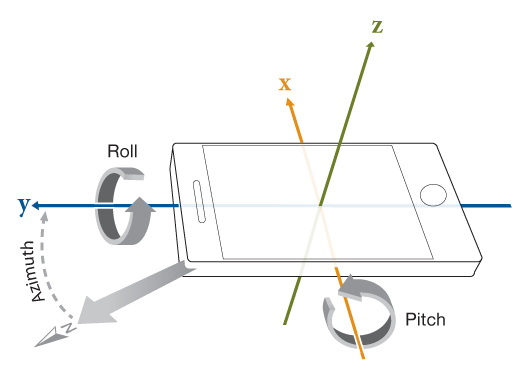
\includegraphics[width=1\linewidth]{az.jpg}
	\caption{Azimuth Pitch e Roll}
	\label{fig:az}
\end{figure}
L'altro sensore utilizzato \'e lo step detector, quest'ultimo informa quando avviene un passo permettendo insieme all'azimuth ottenuto di stimare la posizione del pedone. Di seguito si può vedere il codice relativo al listener che andremo a descrivere ora. Ogni volta che viene rilevato un passo vengono incrementati i valori di step e step2, questi sono dure contatori che servono rispettivamente per il calcolo dei passi prima di richiedere un aggiornamento al GPS e prima di calcolare la velocit\'a, inoltre viene salvato il timestamp di quando \'e avvenuto l'ultimo passo. La velocit\'a viene calcolata ogni cinque passi in quanto il listener non informa dell'avvenimento di un passo in modo immediato ma lo fa in modo non regolare a volte, in questo modo abbiamo un valore approssimato che si avvicina di pi\'u a quello reale. Tale calcolo avviene tramite la formula fisica velocit\'a = spazio / tempo, lo spazio \'e dato dal numero dei passi, nel nostro caso cinque, moltiplicato per la lunghezza del passo, questa lunghezza viene calcolta nel momento in cui viene instaziato l'oggetto della classe HumanLocalService usando il valore dell'altezza dell'utente richiesta in input tramite un dialog, mentre il tempo viene calcolato come il tempo di quando viene effettuato il quinto passo meno quello di quando \'e stato effettuato il primo passo. La velocit\'a che viene restuita infine \'e il massimo tra il valore calcolato e 1, questo serve per riuscire a prevedere quei casi in cui i pedoni si fermano e poi riprendono a camminare all'improvviso. Oltre a ci\'o viene salvato l'azimuth calcolato nel momento in cui \'e stato rilevato un passo e vengono calcolate le nuove coordinate attuali in lat e long conoscendo quelle precedenti, l'angolo rispetto al nord e la lunghezza di un passo. Per quanto riguarda la richiesta delle coordinate reali al GPS essa viene fatta in due casi, se sono stati fatti 30 passi oppure se sono passsati 25 secondi dall'ultimo aggiornamento, in questo modo si cerca di mantenere la posizione accurata. La chiamata al GPS avviene tramite "getCurrentLocation" che aggiorna le coordinate attuali a quelle reali ottenute dal gps, mentre la chiamata ogni 25 secondi avvine tramite l'handler "hnd".  
\begin{lstlisting}
 public void onSensorChanged(SensorEvent sensorEvent) {
    step++;
    step2++;
    timestamp = System.currentTimeMillis();
    if (fst == true) {
        startTime = System.nanoTime();
        fst = false;
    }else if(step2%5==0){
        step2 = 0;
        endTime = System.nanoTime();
        double sp = 5*(stepLength / 100) / ((endTime - startTime) / Math.pow(10, 9));
        speed = Math.max(sp,1);         
        startTime=endTime;
    }
    if (angle != null) {
    azimuth = angolo;
    scX+=(getDistance(
    Math.cos(azimuth))/r_earth)*
    (180/Math.PI)/Math.cos(scY*Math.PI/180);
    scY+=(getDistance(
    Math.sin(azimuth))/r_earth)*
    (180/Math.PI);
    if (step%30==0) {
        hnd.removeCallbacks(rn);
        getCurrentLocation();  
        hnd.postDelayed(rn, 25000);
        }
    }
}
\end{lstlisting}
Un altro parametro calcolato \'e l'accuratezza che viene misurata come la distanza in metri tra la posizione stimata e quella reale ottenuta dal GPS al momento di una chiamata ad esso.

\subsection{Modello di Previsione}
Questo modello viene implementato lato Observer e si occupa di elaborare i dati ricevuti dai diversi Publisher ed incrociarli con quelli del veicolo che rappresenta.
Un modello di previsione prevede come input il tragitto che il veicolo dovra percorrere sottofroma di Polilinea (vettore di segmenti) ed un gestore di posizionamento che sfrutti il segnale GPS in modo da sapere in ogni istante le cordinate attuali del veicolo.
Dati questi input, per ogni Publisher trovato stima se in un tratto della Polilinea di input il veicolo potrebbe andare a collidere con il Publisher. Nel caso lo segnala sulla mappa.
La stima di collisione viene effettuata utilizzando il seguente algoritmo.
 
 
\begin{figure}[h!]
	\centering
	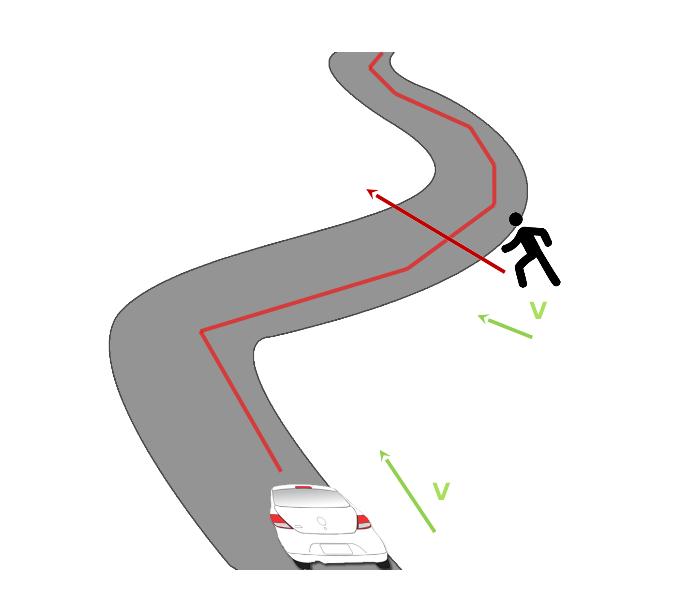
\includegraphics[width=0.7\linewidth]{prevmod}
	\caption{Modello di Previsione}
	\label{fig:prevmod}
\end{figure}
 
Il concetto di fondo \'e che l'uomo collider\'a con il veicolo solo se la sua traiettoria e la sua velocit\'a partendo da un punto A lo porteranno in un punto B tale per cui il segmento AB interseziona uno dei tratti della Polilinea realitiva al tragitto del veicolo.
La seguente funzione verifica se due segmenti si intersezionano.

\begin{lstlisting}
/**
* Check if the human will intersect the vehicle
* @param h human service Object
* @return True -> Intersection
*/
public boolean willHumanIntersectVehicle(HumanService h) 
{
	LatLng loc = getCurrentPosition();
	int start = getCurrentPolylineSegment();
	int end = start;
	// Search indexes on which check intersection
	for(int i = start; i < route.size()-1; i++)
	{
		double d = getPointSegmentProjectionDistance(
			route.get(i),
			route.get(i+1),
			loc);
		if(d < WIFI_MAX_RANGE)
		{
			end = i+1;
		}else{
			break;
		}
	}
	if(end ==  start)
	{
		// All segments are inside 200 meters range
		end = route.size()-1;
	}

	// Intersection check
	for(int i = start; i < end; i++)
	{
		if(doIntersect(
			route.get(i), // P1 of the vehicle
			route.get(i+1), // P2 of the vehicle
			new LatLng(h.latitude, h.longitude), // P1 human
			h.getHumanPositionIn(
			(int) Math.ceil(WIFI_MAX_RANGE / getCurrentSpeed()))  // P2 of the human
		))
		{
		return true;
		}
	}
	return false;       // No intersections
}

\end{lstlisting}
Prima di tutto all'interno di questa funzione viene richiesta la posizione corrente del veicolo ed il segmento di polilinea all'interno del quale esso si trova. Per trovare il segmento di polilinea corrente (funzione \textit{getCurrentPolylineSegment}), viene effettuato un calcolo trigonometrico della distanza tra la posizione del veicolo ed ogni segmento. Successivamente il tratto con la distanza punto-segmento minore e\' considerato quello corrente. La distanza punto-segmento in geometria sferica viene calcolata con il seguente algoritmo. Definiamo con AB il segmento in questione e con C la posizione del veicolo.\\
1) Convertire le coordinate terrestri in coordinate Cartesiane (utilizzando come orgine il centro della terra).\\
2) Calcolare T, il punto sulla retta AB piu\' vicono al  punto C utilizzando i tre seguenti prodotti vettoriali:
\\a) G = A x B\\
b) F = C x G\\
c) T = G x F\\
3) Normalizzare T a moltiplicarlo per il raggio della terra.\\
4) Riconvertire il valore in latitudine e lonfitudine.\\
5) Verificare che il punto si trovi esattamente sul segmento AB, nel caso sovrfascriverlo con l'estremo del segmento piu\' vicino.\\
6) Utilizzare la formula della distanza tra due punti in geometria sferica per trovare la distanza punto-segmento.\\

Proseguento con l'analisi della funzione \textit{willHumanIntersectVehicle}, il primo ciclo for, partendo dal segmento corrente, cerca quali sono i segmenti di polilinea la cui distanza tra segmento e posizione del veicolo risulta essere inferiore al range del WiFi, definito dalla costante WIFI\_MAX\_RANGE. Questo perche\' si presume che il veicolo non possa ricevere un segnale piu\' distante del normale range di trasmissione.
Una volta terminata questa verifica, avremo un estremo superiore ed un estremo inferiore che limitano il numero di indici dei segmenti sui quali poi verra\' eseguito il controllo di intersezione con il segmente pedone.
Il secondo ciclo for esegue per ogni segmento compreso nell intervallo prima definito il controllo di intersezione con il segmento del pedone.
Questo controllo viene eseguito dalla funzione \textit{doIntersect} alla quale vengono passati i due punti del segmento veicolo, la posizione del pedone descritta all'interno del record di Discovery e la stima della posizione del pedone tra J secondi, dove J e\' il tempo impiegato dal veicolo a percorre il range del WiFi.
La nuova posione viene calcolata utilizzando un moto rettilineo uniforme dove il tempo e\' uguale J + timestamp corrent - timestamp\_pos ottenuto dal service discovery del pedone. Timestamp\_pos e\' l'istante in cui e\' stata calcolata la posizione del pedone prima di essere inviata. 
\textit{doIntersect} e\' l'unica funzione ad utilizzare calcoli euclidei invece che sferici. Questo perche\' la superfice di una sfera per porzioni molto piccole, puo\' essere considerata una superficie piana.
Il controllo di intersezione viene sviluppato utilizzato il concetto di orientazione tra punti.
Due segmenti (p1,q1) e (p2,q2) si intersezionano se e solo se una delle seguenti condizione \'e verificata.
\\
1. Caso generale:\\
(p1, q1, p2) e (p1, q1, q2) hanno orientazioni differenti 
\&\& (p2, q2, p1) e (p2, q2, q1) hanno orientazioni differenti.
\\
2. Caso speciale:\\
(p1, q1, p2), (p1, q1, q2), (p2, q2, p1), e (p2, q2, q1) sono collineari \&\& le proiezioni in x di (p1, q1) e (p2, q2) si intersezionano \&\& le proiezioni in y di (p1, q1) e (p2, q2) si intersezionano.
\\
L'insieme di tutti questi algoritmi danno vita al modello di previsione.
 
\begin{figure}[h!]
	\centering
	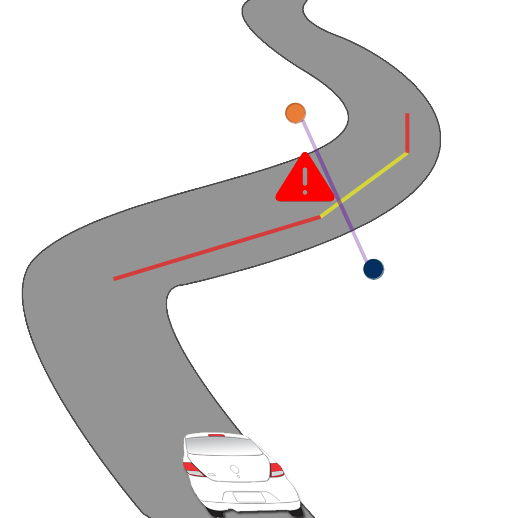
\includegraphics[width=0.7\linewidth]{prevmod1}
	\caption{Intersione tra segmenti}
	\label{fig:prevmod1}
\end{figure}

\section{Valutazione performance}
Sfortunatamente effettuare delle prove con questo sistema non risulta per niente semplice. Questo perche\' sarebbe necessario scegliere un'area urbuana con un alto numero di pedoni e veicoli per intravedere tutti i minimi particolari e poter dunque costruire modelli realistici.
Detto questo, i nostri test sono stati effettuati in aree rurali (per non intralciare il traffico), con pero\'  diversi ostacoli tra trasmettitore e ricevente.
Infatti gli scenarii da noi scelti ed analizzati sono i seguenti.

\begin{center}


	\begin{tabular}{lll|ll}
		\hline
		& \multicolumn{2}{l|}{Sole} & \multicolumn{2}{l}{Pioggia} \\
		& $\bot$        & //        & $\bot$         & //         \\ \hline
		Linea diretta                     & 120m             & X         & 80m              & X          \\ \hline
		\multicolumn{1}{c}{Curva/Ostacoli} & 50m             & X        & 30m             & X         \\ \hline
	\end{tabular}
\\~\\
\textit{Velocit\'a del veicolo $\sim$ 50Km/h}
\\

\end{center}
$\bot$ = Traiettoria pedone $\bot$ traiettoria veicolo.
\\
// = Traiettoria pedone // traiettoria veicolo.
\\
I risultati visulizzati rappresentano i valori  minimi ottenuti su un numero di prove pari a 3.\\
"X" sta a significare "Nessuna segnalazione ricevuta sul dispositivo del veicolo". 
Come si puo' vedere dalla tabella sopra visualizzata, le distanze di preavviso sono notevoli, soprattutto nel caso di spazio aperto (i valori massimi si aggirano sui 160 metri!).
Le distanze di ricezione calano pero' drasticamente nel momento in cui si viaggia in uno spazio urbano (50-30 metri con pioggia). Bisogna per\'o tenere anche in cosiderazione che le velocit\'a in caso di pioggia e paesaggio urbano, soprattutto in prossimit\'a di curve, sarebbero ridotte rispetto a scenari con condizioni pi\'u favorevoli.

\section{Conclusioni}
Il progetto come si puo notare leggendo il documento ha chiaramente delle limitazioni riguardanti principalmente falsi positivi e/o falsi negativi. Supponiamo di avere un pedone che sta proseguendo per la sua strada che attualmente \'e parallela alla nostra ma per una frazione di secondo si gira a salutare un conoscente. In quel momento esatto parte la segnalazione WiFi direct e di conseguenza la traiettoria segnalata nel record di discovery risulta errata, causando in questo modo un avvertimento a tutti i veicoli presenti nella strada adiacente. Questo \'e chiaramente un caso di falso positivo. Attualmente non vi \'e una soluzione a questo problema se non il provare a velocizzare l'update pi\'u rapido sul recod di discovery. Questo per\'o potrebbe causare diversi problemi al driver del modulo WiFi contenuto nel dispositivo. I test da noi effettuati, evidenziano infatti un mancato invio dei dati con tempi di aggiornamento troppo brevi. Ad ogni modo questo problema e relativamente grave, in quanto maggior pericolosit\'a \'e rappresentata dal falso negativo. Un esempio concreto \'e il pedone che ad un certo momento decide di cambiare traiettoria improvvisamente ed attraversare la strada. Questo caso, va analizzato con attenzione. Una possibile soluzione potrebbe essere l'aggiornameto del record di discovery ogni volt\'a che l'orientamento o la velocit\'a cambia (delta \'e maggiore di una soglia) e resta tale per almeno un tempo t. In questo modo i dati rimarrebbero gli stessi per pi\'u tempo limitando gli aggiornamenti inutili, dando invece proirit\'a a quelli utili.
Concludento, il sistema descritto in questo articolo pu\'o essere considerato un punto di partenza. Un ulteriore miglioramento si potrebbe ottenere integrando questo prototipo nel veicolo, migliorando cos\'i le prestazioni del modulo WiFi (antenna con guadagno maggiore).

%% Inserisci bibliografia dei lavori citati (consiglio l'utilizzo di bibtex)
\bibliographystyle{plain}
\begin{thebibliography}{15}

\bibitem{ref1}
\newblock{Subhanjan Saha, Samrat Chatterjee, Amit Kr. Gupta, Indrajit Bhattacharya, Tamal Mondal} 
\newblock{TrackMe - A Low Power Location Tracking System
Using Smart Phone Sensors}
\newblock{\textit{Conference on Computing and Network Communications (CoCoNet'15)}},2015.

\bibitem{ref2}
\newblock{Siim Plangi} 
\newblock{Real-time Localisation and Tracking
System for Navigation Based on Mobile
Multi-sensor Fusion}
\newblock{\textit{UNIVERSITY OF TARTU
Institute of Computer Science}}, 2018.

\bibitem{ref3}
\newblock{Myounggyu Won, Member, IEEE, Ashutosh Mishra, Student Member, IEEE, and Sang H. Son, Fellow, IEEE} 
\newblock{HybridBaro: Mining Driving Routes Using
Barometer Sensor of Smartphone}
\newblock{\textit{IEEE}}, 1558-1748, 2017.


\bibitem{ref4}
\newblock{Wi-Fi Alliance.} 
\newblock{Wi-Fi Peer-to-Peer (P2P)
Technical Specification}
\newblock{\textit{Wi-Fi Alliance}}, 2016.

\end{thebibliography}
\end{document}